\documentclass[12pt]{article}
\usepackage{amssymb,amsfonts,amsmath}
\usepackage{tikz}
\usepackage{pgfplots}
\usetikzlibrary{shapes}




\begin{document}
%\tdplotsetmaincoords{60}{120}
Adapting  the interpretation of 

Indicator Dilution Methods for Measuring Blood Flow, Volume,
and Other Properties of Biological Systems:
A Brief History and Memoir
KENNETH ZIERLER


Consider mass flow, $F[m^3/s]$ through a cylindrical vessel over time $\Delta t [s]$.
For a given concentration, $c[kg/m^3]$, we will define $h(t) [1/s] \Delta t [s]$
as the (mass or volume? ) fraction of the original mass injection, $q_i [kg]$
\[
    q_i [kg] h(t) [1/s] \Delta t [s] \equiv F[m^3/s] c[kg/m^3] \Delta t [s]
    = \text{mass in units of kg flowing out of cylinder}
\]
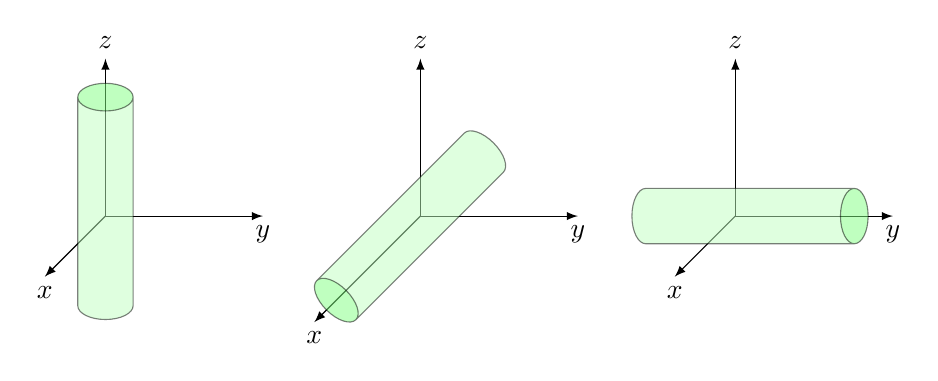
\begin{tikzpicture}

  \coordinate (O) at (0,0,0);
  \coordinate (A) at (2,0,0);
  \coordinate (B) at (0,2,0);
  \coordinate (C) at (0,0,2);

        % draw axis
  \draw[-latex] (O) -- (A) node[below] {$y$};
  \draw[-latex] (O) -- (B) node[above] {$z$};
  \draw[-latex] (O) -- (C) node[below] {$x$};

    \node[cylinder, draw, shape aspect=.5, 
      cylinder uses custom fill, cylinder end fill=green!50, 
      minimum height=1cm,
      cylinder body fill=green!25, opacity=0.5, 
    scale=3, rotate=90]{};

  \begin{scope}[shift={(4,0)}]

    \coordinate (O) at (0,0,0);
    \coordinate (A) at (2,0,0);
    \coordinate (B) at (0,2,0);
    \coordinate (C) at (0,0,3.5);

        % draw axis
    \draw[-latex] (O) -- (A) node[below] {$y$};
    \draw[-latex] (O) -- (B) node[above] {$z$};
    \draw[-latex] (O) -- (C) node[below] {$x$};

    \node[cylinder, draw, shape aspect=.5, 
      cylinder uses custom fill, cylinder end fill=green!50, 
      minimum height=1cm,
      cylinder body fill=green!25, opacity=0.5, 
    scale=3, rotate=-135]{};
  \end{scope}
  \begin{scope}[shift={(8.,0)}]

    \coordinate (O) at (0,0,0);
    \coordinate (A) at (2,0,0);
    \coordinate (B) at (0,2,0);
    \coordinate (C) at (0,0,2);

        % draw axis
    \draw[-latex] (O) -- (A) node[below] {$y$};
    \draw[-latex] (O) -- (B) node[above] {$z$};
    \draw[-latex] (O) -- (C) node[below] {$x$};


    \node[cylinder, draw, shape aspect=.5,  
      cylinder uses custom fill, cylinder end fill=green!50, 
      minimum height=1cm,
      cylinder body fill=green!25, opacity=0.5, 
    scale=3]{};


  \end{scope}


\end{tikzpicture}

With this definition of $h[1/s]$, we can interpret
\[
 F [m^3/s] h(t) [1/s] \Delta t [s] 
\]
as the fraction of  the total flow, $F$ that exists. 
From the geometrical relation, the volume occupied is the length of the cylinder
at time $t$ times the area within the time $t+ \Delta t$.
\[
 \text{distance} =  c [m/s] \cdot t [s]
\qquad
 \text{area} =  \frac{F [m^3/s]}{c[m/s]} 
\]
THus the volume traversed by the mass fraction is the 
\[
 \text{distance * area * mass fraction} =  c [m/s] \cdot t [s]
 \cdot \frac{F [m^3/s]}{c[m/s]}   h(t) [1/s] \Delta t [s] 
  = t F h(t) dt
\]

\end{document}
